\documentclass[border=15pt, multi, tikz]{article}
\usepackage{amssymb}
\usepackage[backend=bibtex,style=authoryear,natbib=true]{biblatex} % Use the bibtex backend with the authoryear citation style (which resembles APA)

\addbibresource{example.bib} % The filename of the bibliography

\usepackage[autostyle=true]{csquotes} % Required to generate language-dependent quotes in the bibliography
\usepackage{import}
\usepackage{tikz}
\usepackage{tikz-network}
\usetikzlibrary{calc,patterns,angles,quotes}
\usepackage{breqn}
\usepackage{bm}
\usepackage{float}
\usepackage{graphicx}
\usepackage{subcaption}
\usepackage{multirow}
\usepackage{graphicx}
\usepackage{rotating}
\usetikzlibrary{fit}
\usetikzlibrary {arrows.meta,graphs,shapes.misc}
\usetikzlibrary {positioning}
\subimport{./layers/}{init}
\newcommand{\bn}{\textbf{n}}
\newcommand{\tabhead}[1]{\textbf{#1}}

\def\ConvColor{rgb:yellow,5;red,2.5;white,5}
\def\ConvReluColor{rgb:yellow,5;red,5;white,5}
\def\PoolColor{rgb:red,1;black,0.3}
\def\DcnvColor{rgb:blue,5;green,2.5;white,5}
\def\SoftmaxColor{rgb:magenta,5;black,7}
\def\SumColor{rgb:blue,5;green,15}
\def\poolsep{1}


\begin{document}
	
The approaches are trained on dataset "synthetic-50-5" as mentioned in Chapter \ref{ch:04} with 3000 scenes. The input matrix has $ 128\times 128 $ height and width. Each vertex map has dimension $ 128\times 128\times3 $, light map has $ 128\times 128 \times 3 $, image has dimension $ 128\times 128 \times 1 $. The model is trained with PyTorch 1.10.0a0, CUDA 11.4.1, GPU with single NVIDIA GEFORCE RTX 3090.


\section{GCNN model evaluation}
The GCNN model is the base model of the whole thesis. In this section, we first evaluate the inpainting performance of the model based on light map input. Then we use the same model for normal inference task.


\subsection{Light Inpainting}
The light inpainting task in this section in order to evaluate the noise inpainting performance of GCNN model. It takes semi-dense light map as input to predict the fully dense light map, as shown in Figure \ref{fig:light-net-archi}.

\begin{figure}[th]
	\centering
	%% https://tex.stackexchange.com/questions/12020/what-is-the-easiest-way-to-draw-a-3d-cube-with-tikz
	\begin{tikzpicture}
		%% -------------------------------------- parameters ------------------------------------------------
		\pgfmathsetmacro{\vdist}{0.4}
		
		\pgfmathsetmacro{\boxsizea}{2}	%% width 512
		\pgfmathsetmacro{\boxwidtha}{2}	%% width 3
		
		%% https://www.tug.org/pracjourn/2007-4/walden/color.pdf
		\definecolor{netcolor}{rgb}{0.5,0.7,0.7}
		
		%% 	d_in							3x512x512
		%%	dconv1: 	d_in-->x1 			32x512x512
		\pgfmathsetmacro{\disttimes}{1}	%% width 32
		\pgfmathsetmacro{\yshift}{1}	%% width 32
		\pgfmathsetmacro{\boxsize}{\boxsizea}	%% size 512
		\pgfmathsetmacro{\boxwidth}{\boxwidtha}	%% width 32
		\pgfmathsetmacro{\yschift}{-1}
		
		
		\node[inner sep=0pt] (input) at (\vdist*\disttimes-6,\yschift-0.8)
		{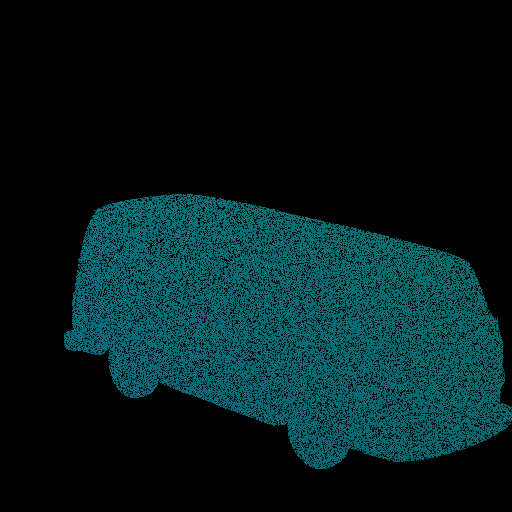
\includegraphics[width=.2\textwidth]{./Figures/gcnn-synthetic/intrinsic_image_light_input.png}};
		\node[text width=3.5cm] at (\vdist*\disttimes-6,\yschift-2.4) {Semi-dense Light Map};
		
		\node[inner sep=0pt] (output) at (\vdist*\disttimes+3,\yschift-0.8)
		{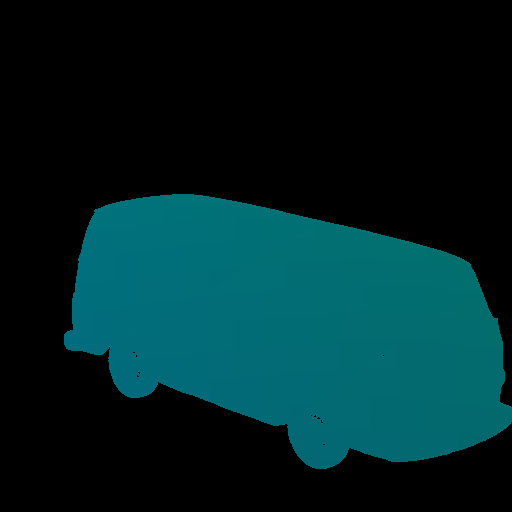
\includegraphics[width=.2\textwidth]{./Figures/gcnn-synthetic/intrinsic_image_light.png}};
		\node[text width=3.5cm] at (\vdist*\disttimes+3,\yschift-2.4) {fully-dense Light Map};
		
		\draw [-stealth] (\vdist*\disttimes-4.5,\yschift-1) -- (\vdist*\disttimes-3.5,\yschift-1);
		\draw [-stealth] (\vdist*\disttimes,\yschift-1) -- (\vdist*\disttimes+1,\yschift-1);
		
		
		\pgfmathsetmacro{\disttimes}{-2}	%% width 32		
		\pgfmathsetmacro{\yschift}{-1}
		\draw[black, fill=netcolor] (\vdist*\disttimes,\yschift,0) -- ++(-\boxwidth,0,0) -- ++(0,-\boxsize,0) -- ++(\boxwidth,0,0) -- cycle;
		\draw[black, fill=netcolor] (\vdist*\disttimes,\yschift,0) -- ++(0,0,-\boxsize) -- ++(0,-\boxsize,0) -- ++(0,0,\boxsize) -- cycle;
		\draw[black, fill=netcolor] (\vdist*\disttimes,\yschift,0) -- ++(-\boxwidth,0,0) -- ++(0,0,-\boxsize) -- ++(\boxwidth,0,0) -- cycle;
		
		\node[text width=3.5cm] at (\vdist*\disttimes+0.3,\yschift-1) {GCNN};
	\end{tikzpicture}
	\caption{Light map inpainting based on GCNN architecture.}
	\label{fig:light-net-archi}
\end{figure}

The network is trained on 3000 light maps in the "synthetic-50-5" dataset with initial learning rate 0.001, learning schedule 8,1000 with decay factor 0.5, the batch size is 8, the feature map channel is 128 in all of the gated convolution layers. The result is shown in Table \ref{tab:light-inpainting}


\begin{table}[th]
	
	\centering
	\begin{tabular}{l l l l l l l l }
		\tabhead{Model} & \tabhead{Angle} & \tabhead{Time /ms} & \tabhead{bz} & \tabhead{lr-schedule} & \tabhead{lr-df} & \tabhead{l/i. Nr.} & over-perform\\
		LightNet  & 0.17  & 4.72 & &  & & & \\ 
		\hline
		GCNN  & 10.57 & 5.25 & 8 & 200,1600 & 0.5 & 0 & - \\
		\hline
		an3 & 10.46 & 64.86 & 8 & 3,12,1000  & 0.5 & 1 & yes\\
		\hline
		an3 & 10.81 & 65.34 & 8 & 10,1000  & 0.5 & 1 & no(yes) \\
		\hline
		VIL-1 & 10.50 & 31.57 & 8 & 10,1000 & 0.5 & 1 & yes \\
		\hline
		VIL-1 & 10.82 & 32.61 & 8 & 3,12,1000 & 0.5 & 1 & no(yes) \\
		\hline
		VIL-3  & 10.79 & 54.76 & 8 & 100,1000 & 0.1 & 3 & no(yes) \\
		\hline
		VIL-10  & 11.10 & 132.32 & 8 & 100,1000 & 0.1 &10 & no(yes)\\
	\end{tabular}
	\caption{The error of models. The angle error is the average angle error of all valid pixels in the test case. The time unit is millisecond. bz is the batch size, lr-schedule is learning rate schedule. lr-df is learning rate decay factor, l/i. Nr is the number of light-image maps used for each scene}	
	\label{tab:light-inpainting}
\end{table}


%% nnnn exp
\section{Surface Normal Inference based on Depth Map}
The goal of surface normal inference is to calculate the tangent surface normal map $ N $ from a single depth map $ D $. A network named Gated Convolution Neural Network (GCNN) ( \ref{gcnn}) is trained and is compared with similar approaches. We evaluate the performance of the model in dataset ``synthetic50-5" introduced in  \ref{ch:04} including 5K depth maps with size  $ 512\times512\times3 $ for training. All the depth maps add simulated noise as introduced in \ref{sec:noise}. The training pipeline use batch size $ 8 $,  Adam optimizer (\cite{adam}), learning rate of  $ 1\times10^{-3} $, penalty-l2 loss. The output is directly the tangent normal in range $ \left[-1,1\right] $. The output and input has the same shape. 

\subsection{Qualitative Evaluation}

The evaluation visualization on test dataset is shown in Figure \ref{fig:gcnn-eval-synthetic}. As shown in the picture, GCNN model 
Figure \ref{fig:gcnn-eval-synthetic-zoom-in} zooms in the hindhead area of the dragon object which provides a closer comparison with the ground-truth.
\begin{figure}[th]
	\centering
	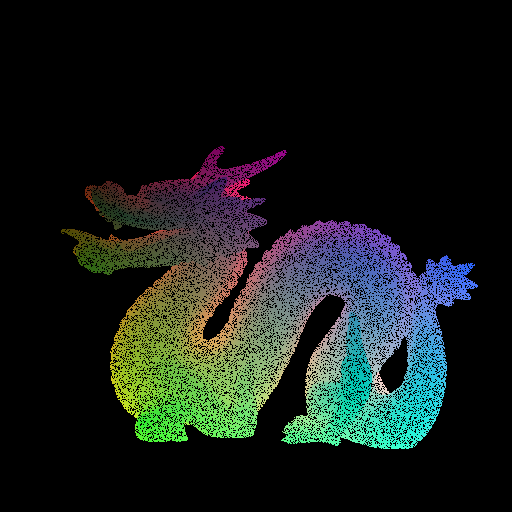
\includegraphics[width=0.15\linewidth]{./Figures/comparison/fancy_eval_6_point_cloud_noise.png}
	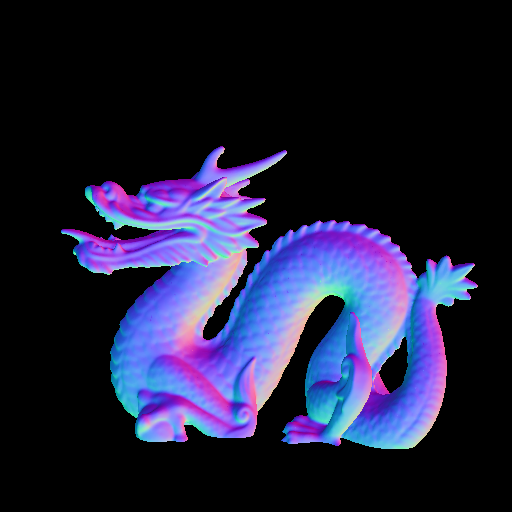
\includegraphics[width=0.15\linewidth]{./Figures/comparison/fancy_eval_6_groundtruth.png}
	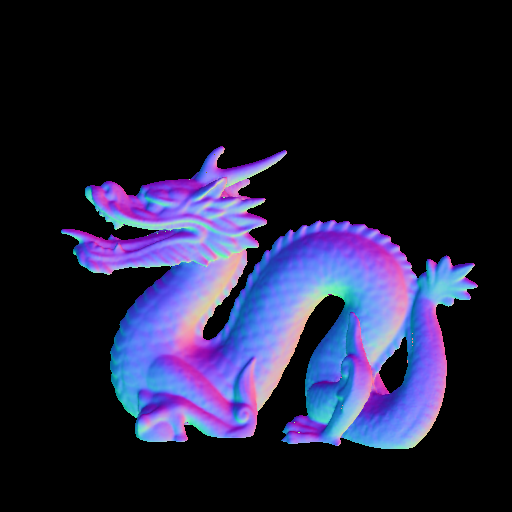
\includegraphics[width=0.15\linewidth]{./Figures/comparison/fancy_eval_6_normal_GCNN3-32-512.png}
	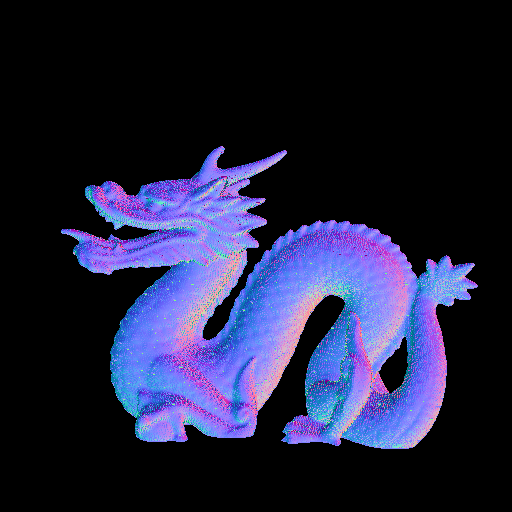
\includegraphics[width=0.15\linewidth]{./Figures/comparison/fancy_eval_6_normal_SVD.png}
	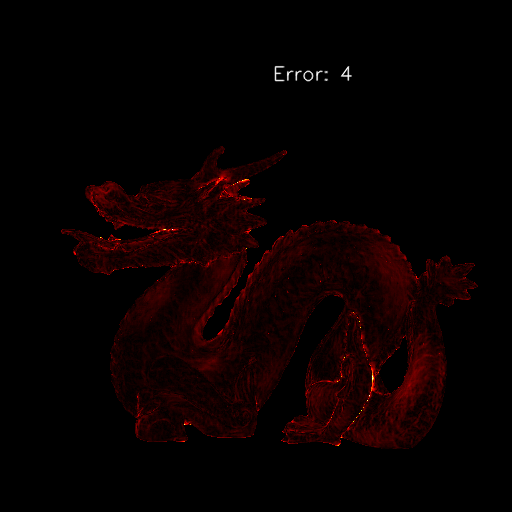
\includegraphics[width=0.15\linewidth]{./Figures/comparison/fancy_eval_6_error_GCNN3-32-512.png}
	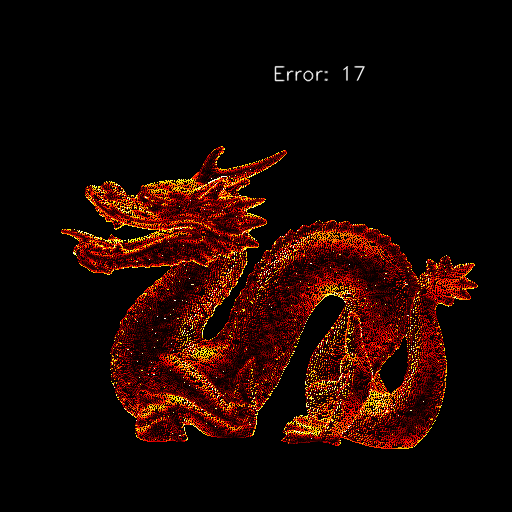
\includegraphics[width=0.15\linewidth]{./Figures/comparison/fancy_eval_6_error_SVD.png}
	\caption{GCNN Normal Inference on Synthetic Dataset (object: dragon) From left to right: Input vertex map, ground-truth, GCNN normal map, SVD normal map, GCNN error map, SVD error map}
	\label{fig:gcnn-eval-synthetic}
\end{figure}



\begin{figure}[th]
	\centering
	\begin{subfigure}[b]{0.15\linewidth}
		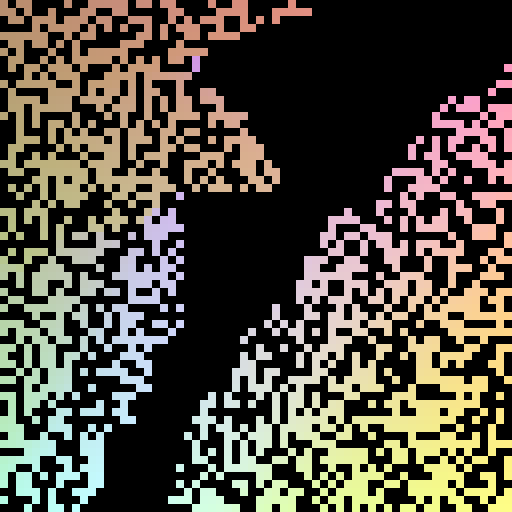
\includegraphics[width=\linewidth]{./Figures/comparison/eval_2_input.png}
		\caption{Input}
	\end{subfigure}
	\begin{subfigure}[b]{0.15\linewidth}
		
\includegraphics[width=\linewidth]{./Figures/comparison/eval_2_normal_GT.png}
		\caption{GT}
	\end{subfigure}
	\begin{subfigure}[b]{0.15\linewidth}
		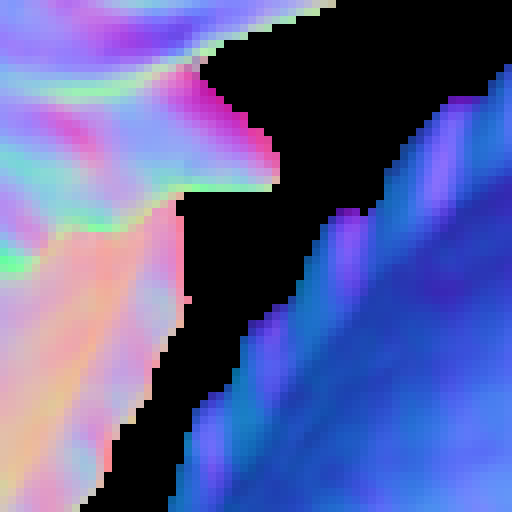
\includegraphics[width=\linewidth]{./Figures/comparison/eval_2_normal_GCNN.png}
		\caption{GCNN}
	\end{subfigure}
	\begin{subfigure}[b]{0.15\linewidth}
		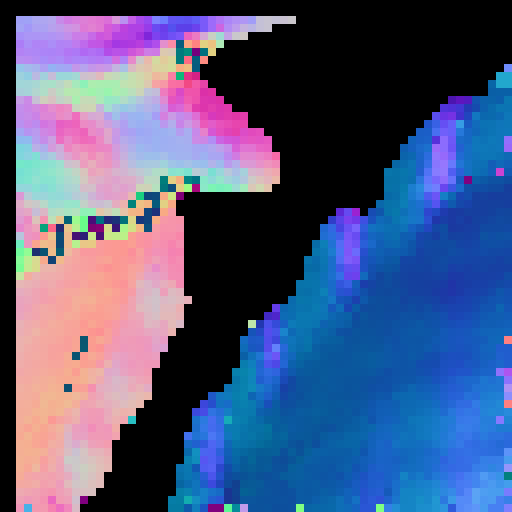
\includegraphics[width=\linewidth]{./Figures/comparison/eval_2_normal_SVD.png}
		\caption{SVD}
	\end{subfigure}
	\begin{subfigure}[b]{0.15\linewidth}
		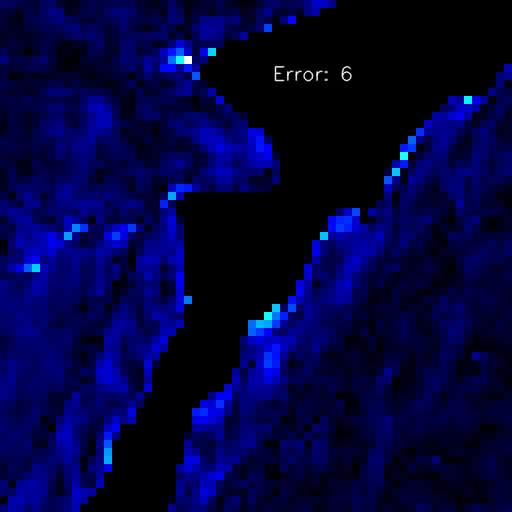
\includegraphics[width=\linewidth]{./Figures/comparison/eval_2_error_GCNN.png}
		\caption{}
	\end{subfigure}
	\begin{subfigure}[b]{0.15\linewidth}
		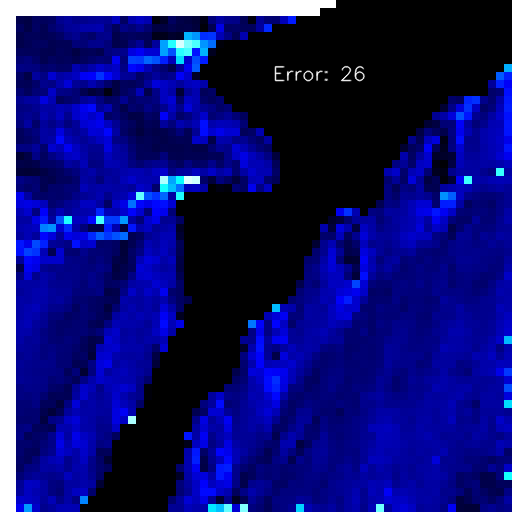
\includegraphics[width=\linewidth]{./Figures/comparison/eval_2_error_SVD.png}
		\caption{}
	\end{subfigure}
	\caption{Zoom in of dragon object evaluation.}
	\label{fig:gcnn-eval-synthetic-zoom-in}
\end{figure}



The evaluation visualization on real dataset is shown in Figure \ref{fig:gcnn-eval-real}
\begin{figure}[th]
	\centering
	\begin{subfigure}[b]{0.24\linewidth}
		
\includegraphics[width=\linewidth]{./Figures/gcnn-real/fancy_eval_1_point_cloud_noise.png}
		\caption{point cloud}
	\end{subfigure}
	\begin{subfigure}[b]{0.24\linewidth}
		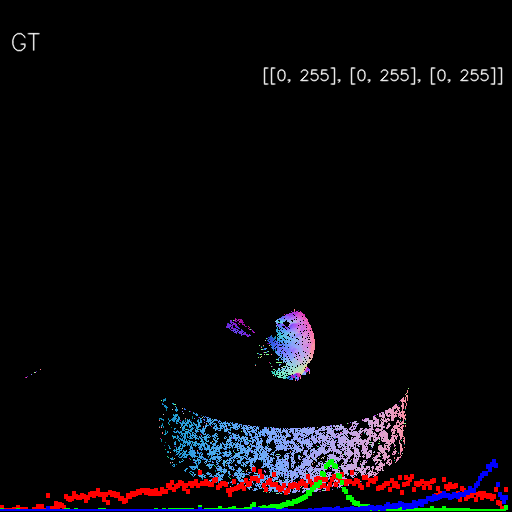
\includegraphics[width=\linewidth]{./Figures/gcnn-real/fancy_eval_1_groundtruth.png}
		\caption{ground-truth}
	\end{subfigure}
	\begin{subfigure}[b]{0.24\linewidth}
		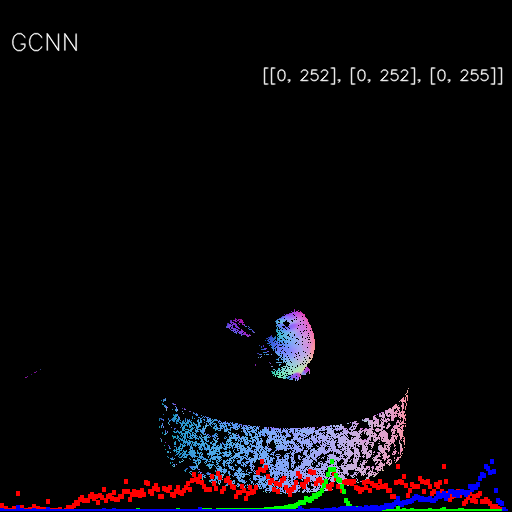
\includegraphics[width=\linewidth]{./Figures/gcnn-real/fancy_eval_1_normal_GCNN.png}
		\caption{GCNN}
	\end{subfigure}
	\begin{subfigure}[b]{0.24\linewidth}
		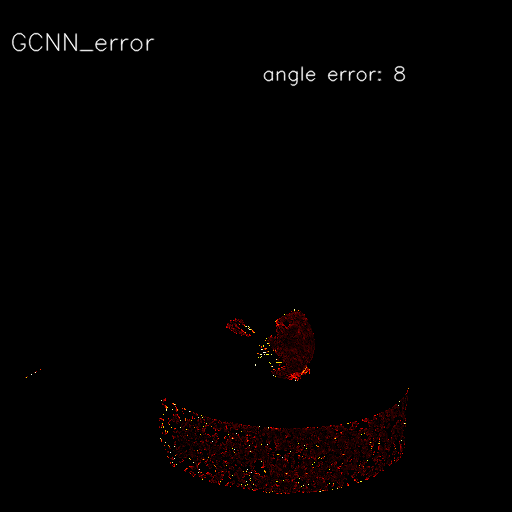
\includegraphics[width=\linewidth]{./Figures/gcnn-real/fancy_eval_1_error_GCNN.png}
		\caption{Angle Error}
	\end{subfigure}
	\caption{Evaluation on Real Dataset}
	\label{fig:gcnn-eval-real}
\end{figure}



\subsection{Quantitative Evaluation }





The evaluation result on test scenes is shown in Figure \ref{fig:scatter-gcnn}.
The GCNN based method has angle error between 5 to 15 degrees in both type of inputs. The error trends to higher with point number decrease. It is because the less points in the point cloud, the more detail is hided due to the insufficient of resolution. Therefore the recorded surface based on the point cloud is more coarse, which also increase the difficulty of the normal inference.

\begin{figure}[h!]
	\centering
	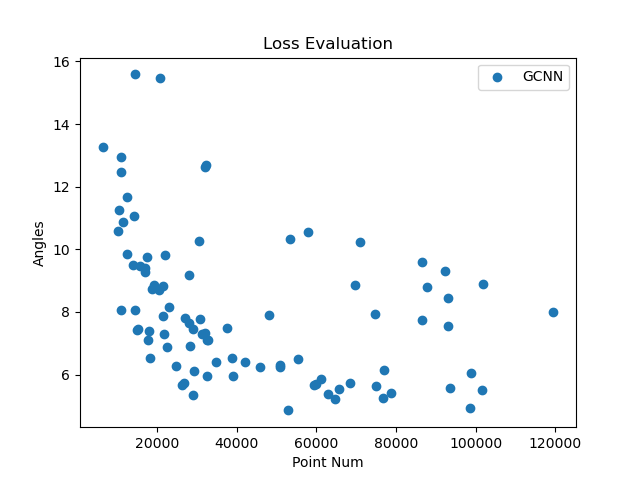
\includegraphics[width=.4\textwidth]{./Figures/scatter-gcnn-no-noise.png}
	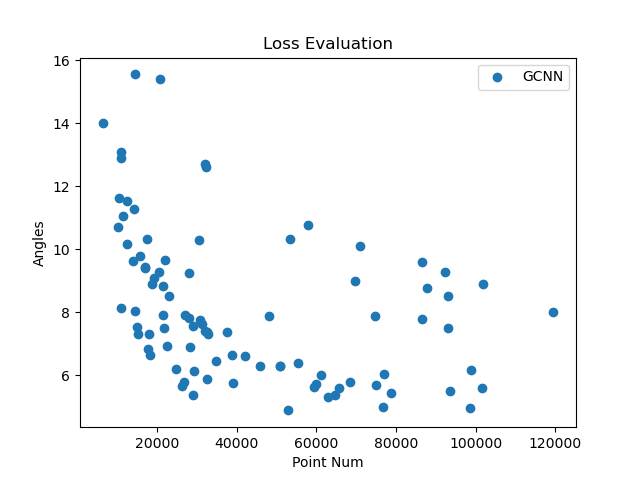
\includegraphics[width=.4\textwidth]{./Figures/scatter-gcnn-noised.png}
	\caption{Evaluation of average angular loss on the whole test dataset with 90 scenes. The x-axis indicates the point number, the y-axis indicates the angles. The \textbf{Left} one using point cloud without noise, the \textbf{right} one has noise.}
	\label{fig:scatter-gcnn}
\end{figure}




\subsection{Speed}




\section{Guided Gated Convolution Neural Network for Normal Inference }

\subsection{Light Net Evaluation}

We evaluate the GCNN architecture based light net on the test dataset. The light net parameters are further used as the initial parameter of light branch of the Trignet.

A qualitative evaluation of light net is shown in Figure \ref{fig:eval-light}. The average angular error are lower than $ 0.3 $ degree on all of test cases. In this case, to distinguish the output and the ground truth is already not easily only use naked eyes. 


\begin{figure}[th]
	\centering
	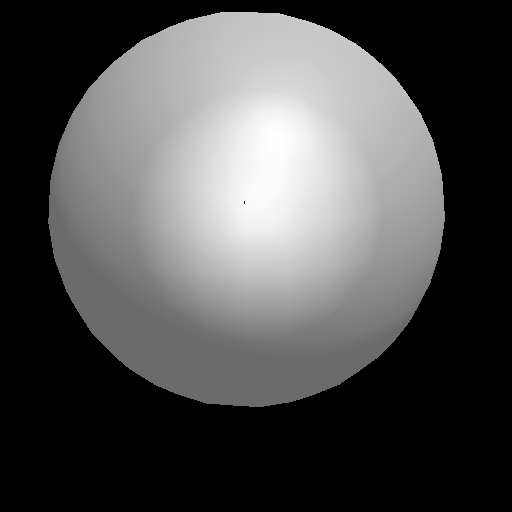
\includegraphics[width=0.18\linewidth]{./Figures/light-synthetic/fancy_eval_0_img.png}
	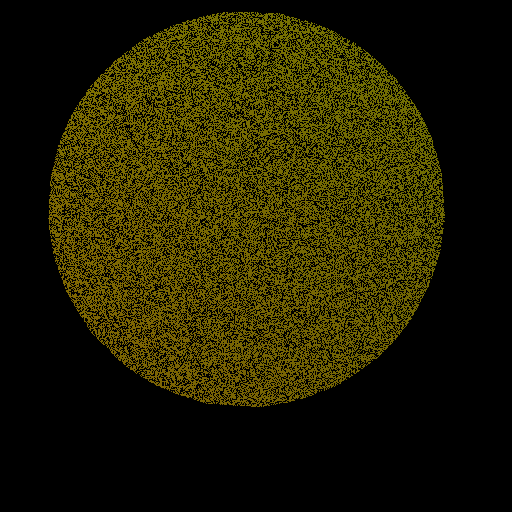
\includegraphics[width=0.18\linewidth]{./Figures/light-synthetic/fancy_eval_0_light_input.png}
	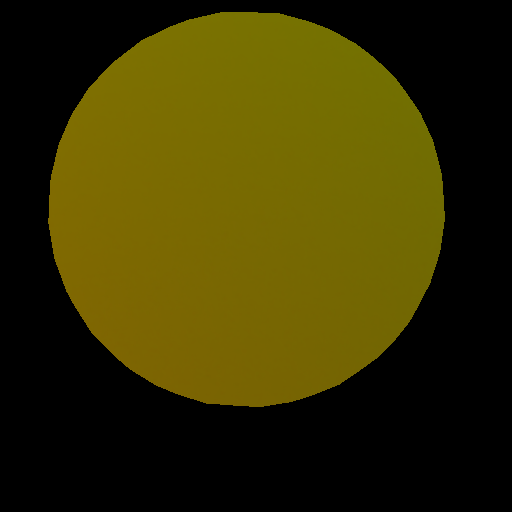
\includegraphics[width=0.18\linewidth]{./Figures/light-synthetic/fancy_eval_0_light_light.png}
	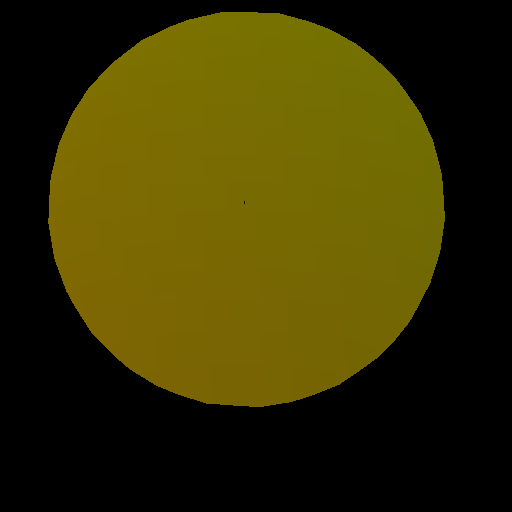
\includegraphics[width=0.18\linewidth]{./Figures/light-synthetic/fancy_eval_0_light_gt.png}
	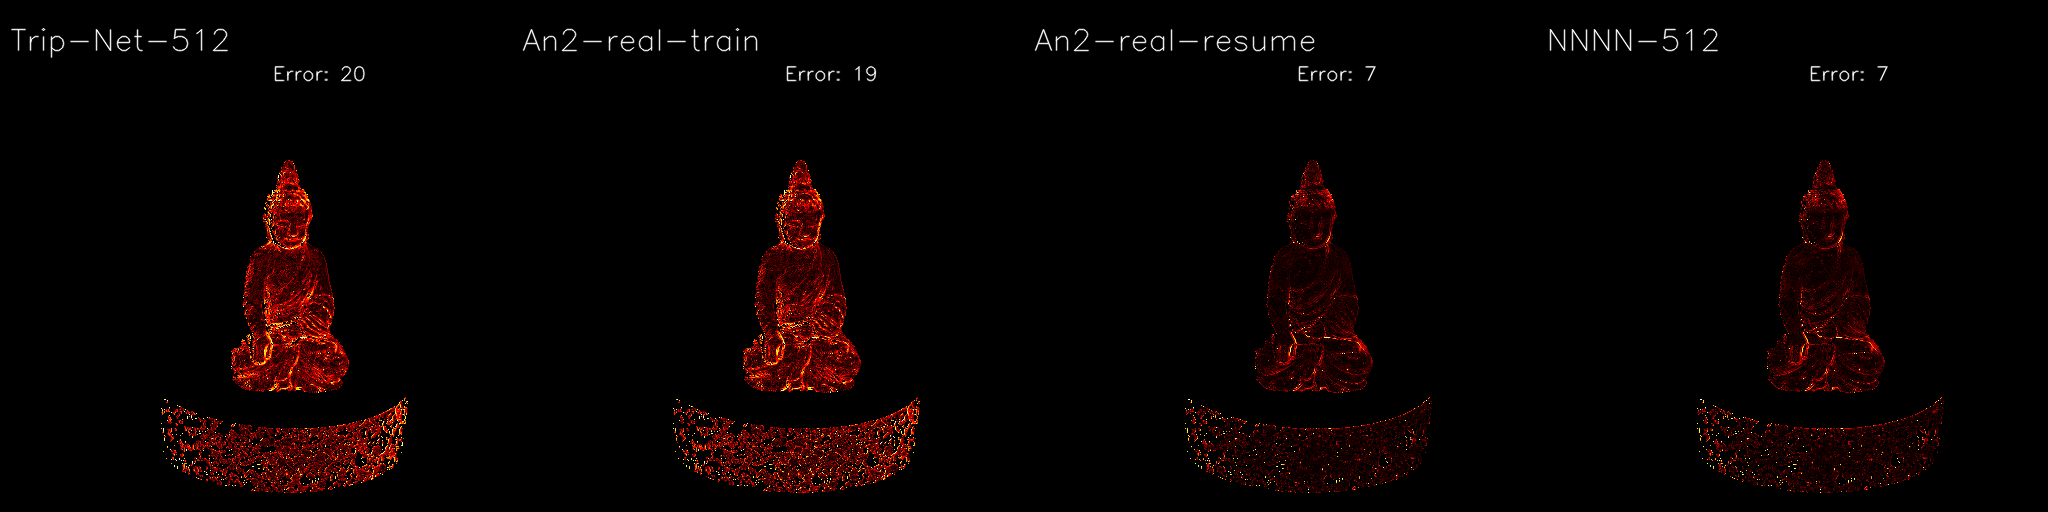
\includegraphics[width=0.18\linewidth]{./Figures/light-synthetic/fancy_eval_0_output_error.png}
	
	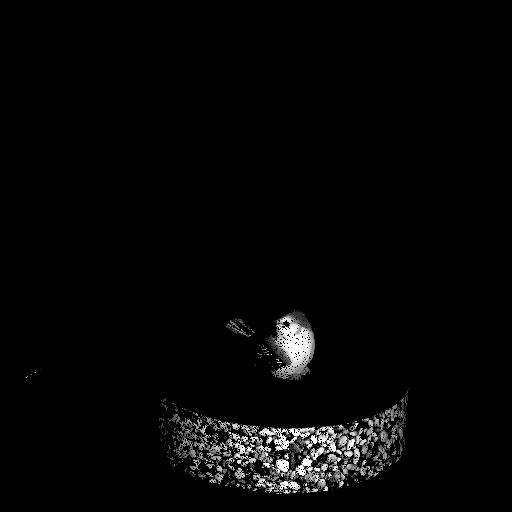
\includegraphics[width=0.18\linewidth]{./Figures/light-synthetic/fancy_eval_1_img.png}
	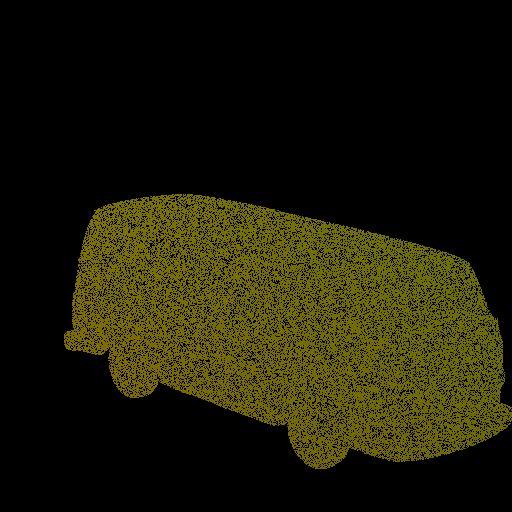
\includegraphics[width=0.18\linewidth]{./Figures/light-synthetic/fancy_eval_1_light_input.png}
	
\includegraphics[width=0.18\linewidth]{./Figures/light-synthetic/fancy_eval_1_light_light.png}
	
\includegraphics[width=0.18\linewidth]{./Figures/light-synthetic/fancy_eval_1_light_gt.png}
	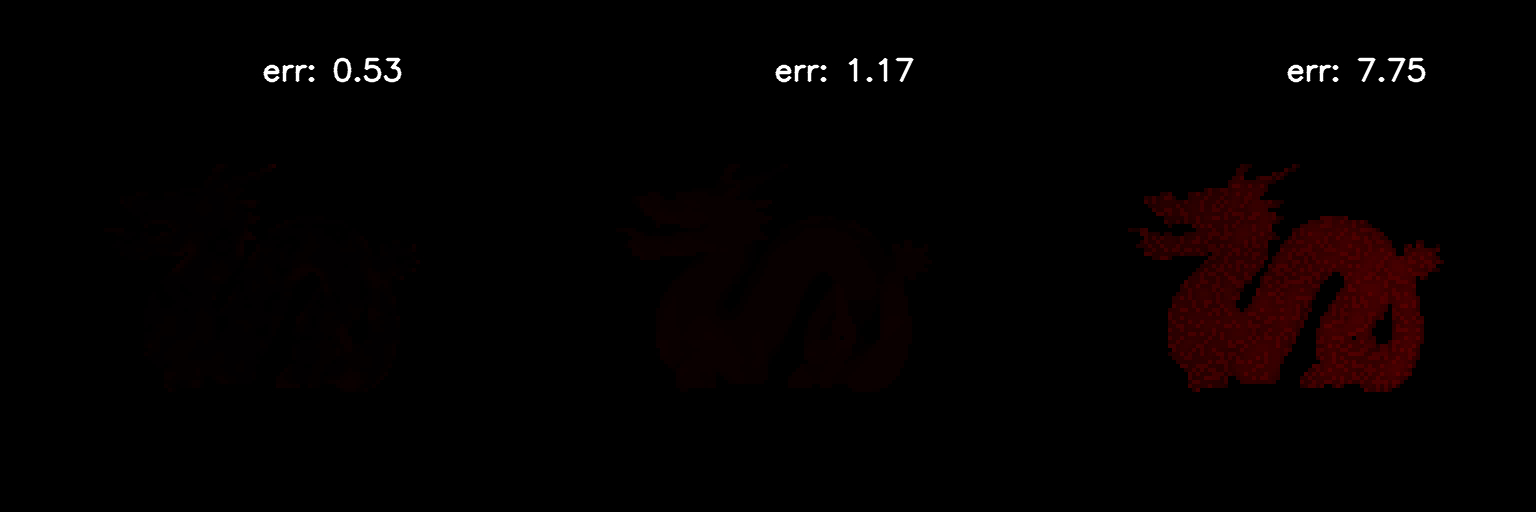
\includegraphics[width=0.18\linewidth]{./Figures/light-synthetic/fancy_eval_1_output_error.png}
	
	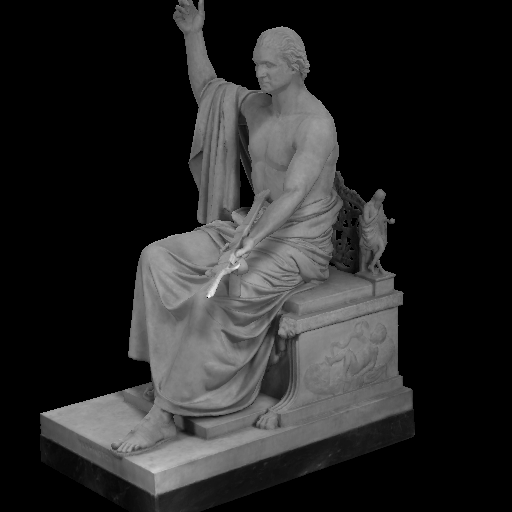
\includegraphics[width=0.18\linewidth]{./Figures/light-synthetic/fancy_eval_4_img.png}
	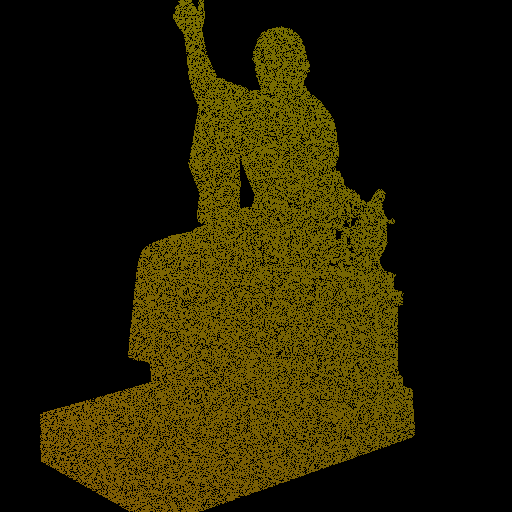
\includegraphics[width=0.18\linewidth]{./Figures/light-synthetic/fancy_eval_4_light_input.png}
	
\includegraphics[width=0.18\linewidth]{./Figures/light-synthetic/fancy_eval_4_light_light.png}
	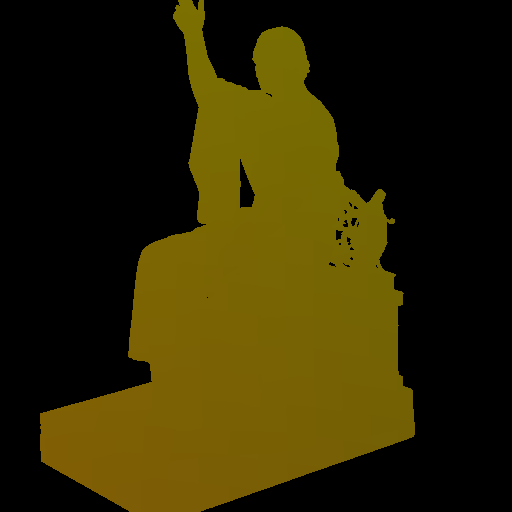
\includegraphics[width=0.18\linewidth]{./Figures/light-synthetic/fancy_eval_4_light_gt.png}
	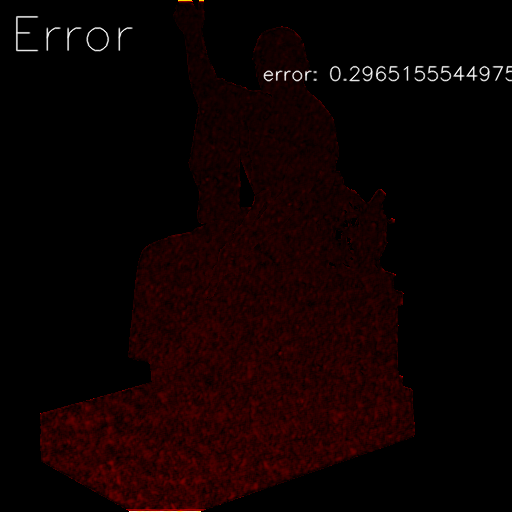
\includegraphics[width=0.18\linewidth]{./Figures/light-synthetic/fancy_eval_4_output_error.png}
	
	\caption{Qualitative evaluation of light net on Sphere, bus and Washington statue. From left to right, grayscale image, semi-dense light map(input), full-dense light map(output), full-dense light map(ground-truth), error map.}
	\label{fig:eval-light}
\end{figure}

Figure \ref{fig:scatter-light} uses a scatter plot to show the average angular error on 100 different test cases. The average pixel-wise angular error is 0.17 degree as shown in Table \ref{tab:model-error}. An regression line has been added in the plot to analysis the tendency of the errors. The angular error slightly goes up when valid point number in the scene increase. It is make sense since the valid pixels are usually connected and concentrate in a single patch, the less of the area of the patch, which corresponding the number of the valid points, the less variation of the light direction among the pixels, thus better the evaluation.


\begin{figure}[th]
	\centering
	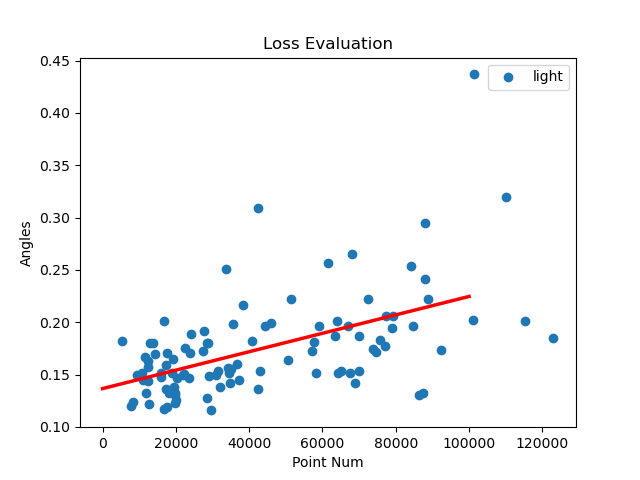
\includegraphics[width=0.5\linewidth]{./Figures/scatter-light-noised.png}
	\caption{The evaluation on 100 test cases of Light Net.}
	\label{fig:scatter-light}
\end{figure}



\subsection{Vertex-Image-Light Net (VIL Net) Evaluation}


The qualitative evaluation of VIL net uses the model trained based on masked L2 loss.

\subsubsection{title}

\begin{figure}[th]
	\centering
	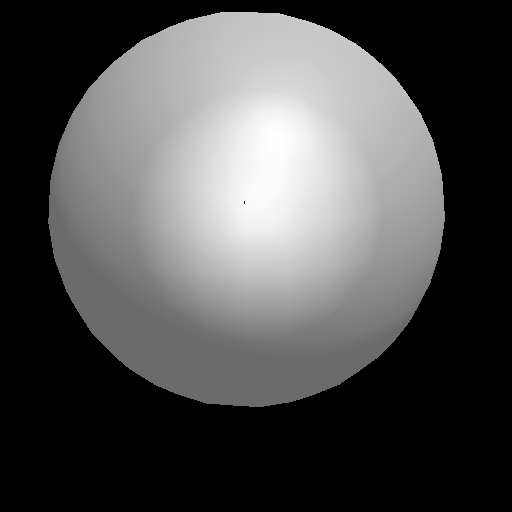
\includegraphics[width=0.18\linewidth]{./Figures/light-synthetic/fancy_eval_0_img.png}
	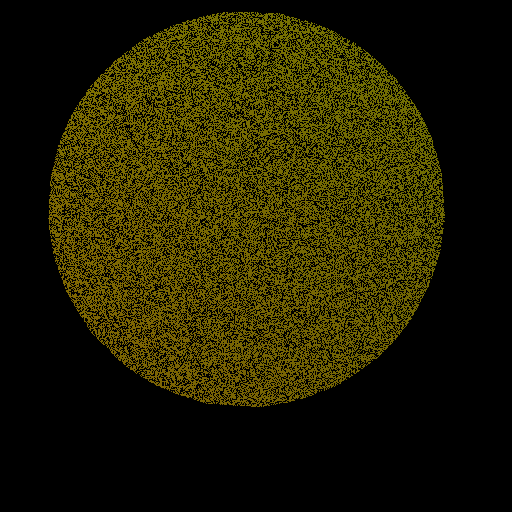
\includegraphics[width=0.18\linewidth]{./Figures/light-synthetic/fancy_eval_0_light_input.png}
	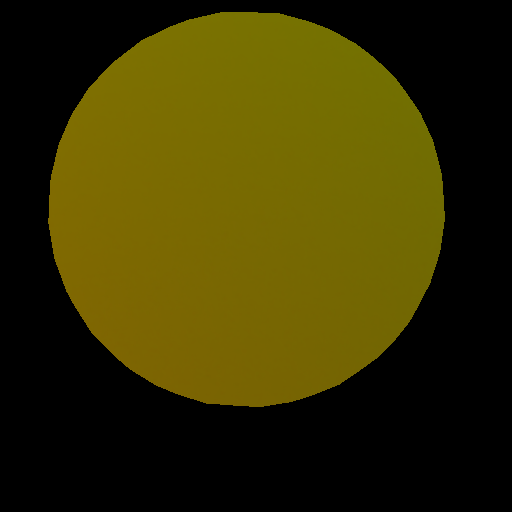
\includegraphics[width=0.18\linewidth]{./Figures/light-synthetic/fancy_eval_0_light_light.png}
	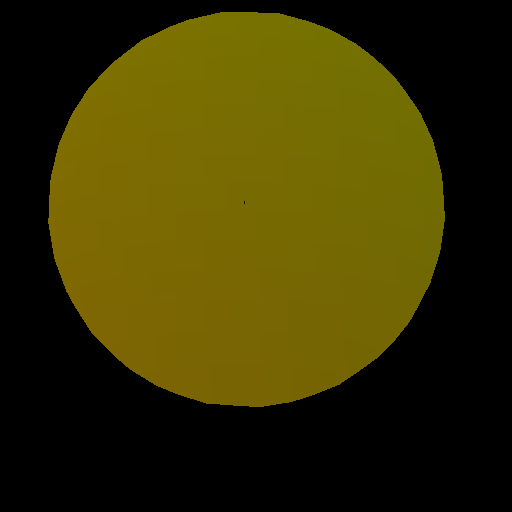
\includegraphics[width=0.18\linewidth]{./Figures/light-synthetic/fancy_eval_0_light_gt.png}
	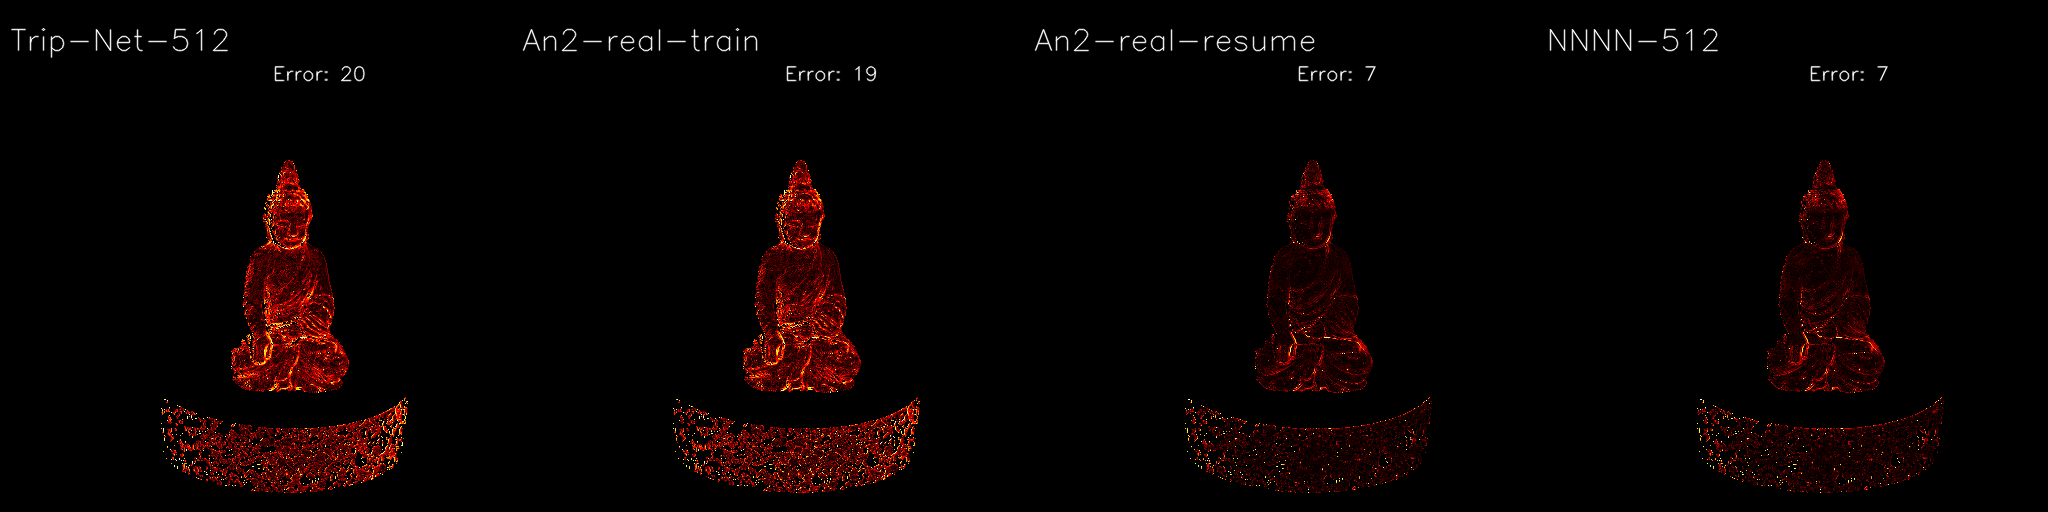
\includegraphics[width=0.18\linewidth]{./Figures/light-synthetic/fancy_eval_0_output_error.png}
	
	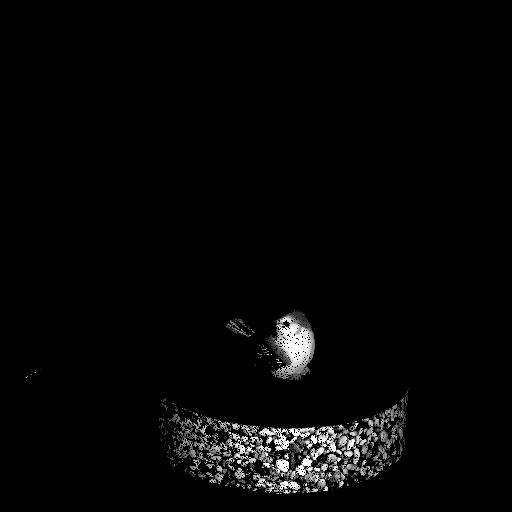
\includegraphics[width=0.18\linewidth]{./Figures/light-synthetic/fancy_eval_1_img.png}
	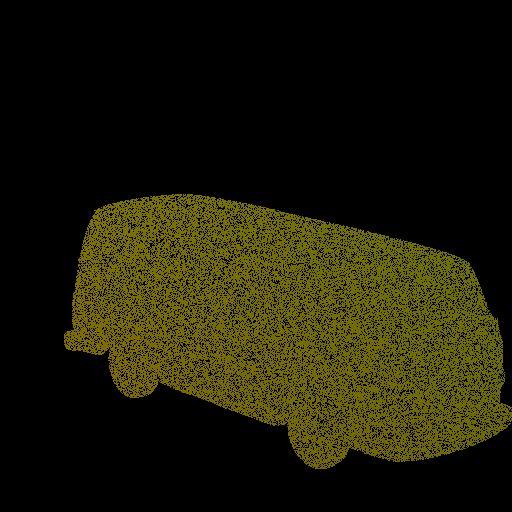
\includegraphics[width=0.18\linewidth]{./Figures/light-synthetic/fancy_eval_1_light_input.png}
	
\includegraphics[width=0.18\linewidth]{./Figures/light-synthetic/fancy_eval_1_light_light.png}
	
\includegraphics[width=0.18\linewidth]{./Figures/light-synthetic/fancy_eval_1_light_gt.png}
	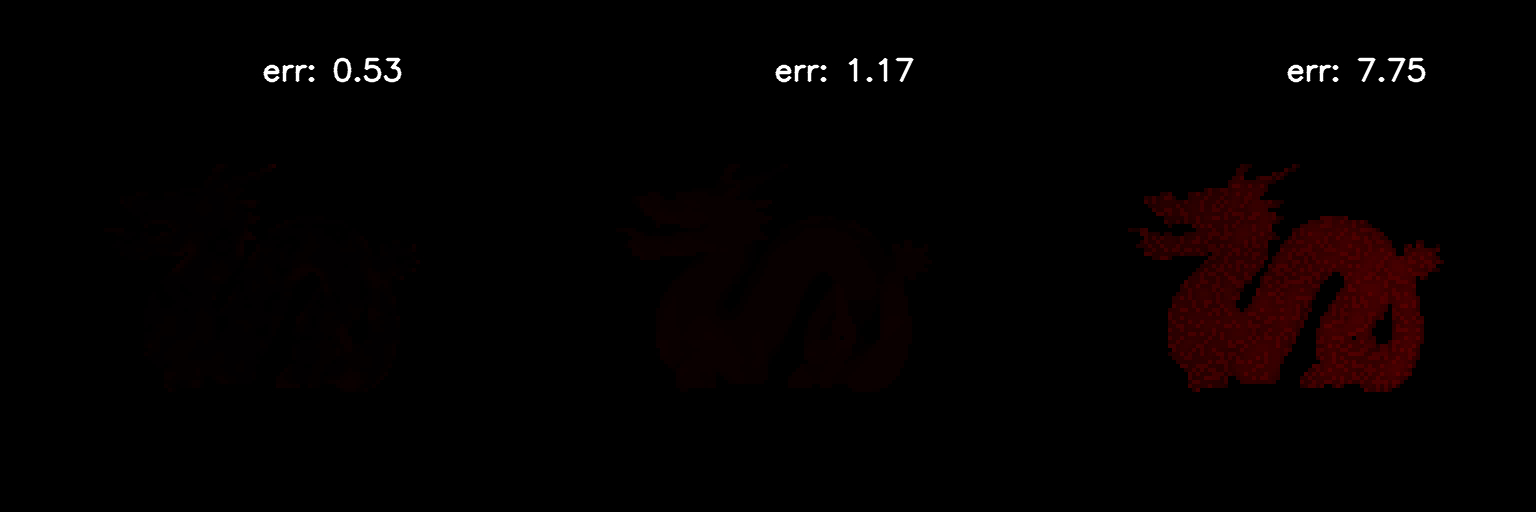
\includegraphics[width=0.18\linewidth]{./Figures/light-synthetic/fancy_eval_1_output_error.png}
	
	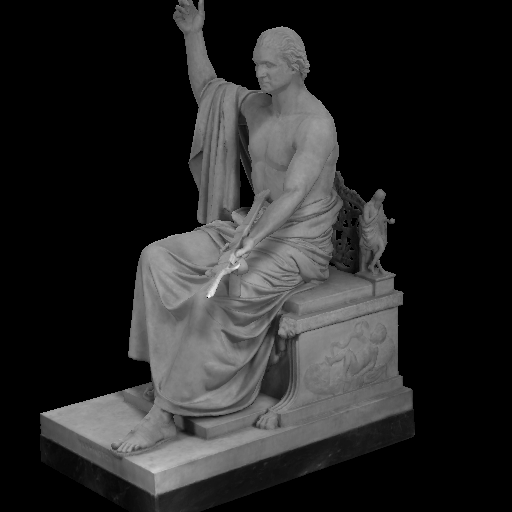
\includegraphics[width=0.18\linewidth]{./Figures/light-synthetic/fancy_eval_4_img.png}
	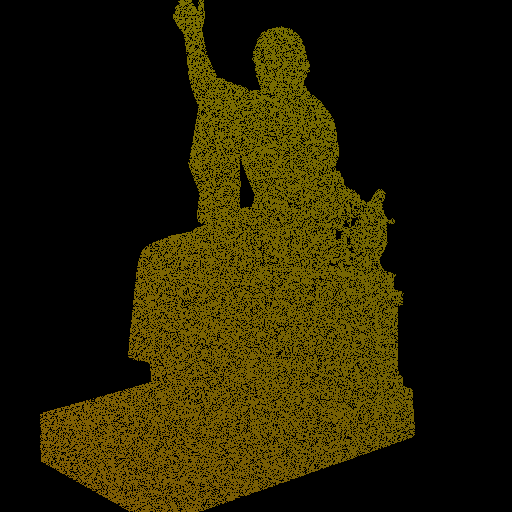
\includegraphics[width=0.18\linewidth]{./Figures/light-synthetic/fancy_eval_4_light_input.png}
	
\includegraphics[width=0.18\linewidth]{./Figures/light-synthetic/fancy_eval_4_light_light.png}
	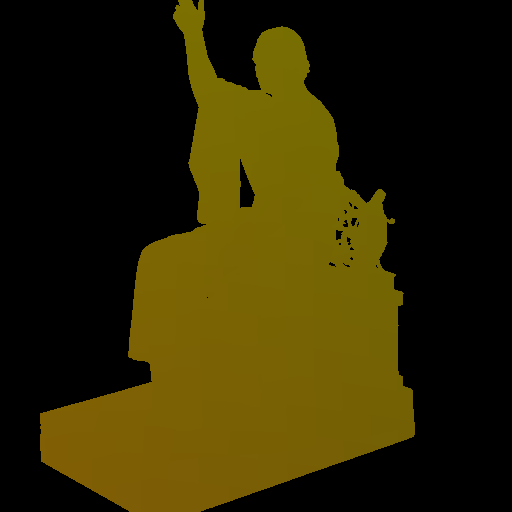
\includegraphics[width=0.18\linewidth]{./Figures/light-synthetic/fancy_eval_4_light_gt.png}
	\includegraphics[width=0.18\linewidth]{./Figures/light-synthetic/fancy_eval_4_output_error.png}
	
	\caption{Qualitative evaluation of Trignet net on Sphere, bus and Washington statue. From left to right, semi 3D vertex map, full-dense normal map(output), full-dense normal map(ground-truth), error map.}
	\label{fig:eval-trignet}
\end{figure}

\begin{figure}[th]
	\centering
	\includegraphics[width=0.5\linewidth]{./Figures/scatter-light-noised.png}
	\caption{The evaluation on 100 test cases of Trignet.}
	\label{fig:scatter-trignet}
\end{figure}




\subsection{comparison}
From the Figure \ref{fig:normal-histo-diff} we can observe the normal difference between ground-truth and GCNN predicted normals in another dimension. It separates the interval $ \left[ -1,1 \right] $, which is exactly the range of normal vector, to 256 sections. Then it counts the number of points locates in each section for 3 axes.  The 3 axes are fitted quite well in most of interval but other than $ \left[ -0.25,0.25 \right] $ for x and y axes and  interval close to $ -1 $ for z axis. Therefore a further constraint can be considered to the loss function related to the normal difference shown in this figure.

It is faulty that almost no normal has -1 z-component in GCNN predicted normal map. The reason?
\begin{figure}[th]
	\centering
	\includegraphics[width=\linewidth]{./Figures/normal-histo-diff.png}
	\caption{The normal difference of between GCNN and ground-truth in x, y, z-axis respectively. The y axis indicates the number of points, x axis indicates the value of normal in x/y/z axis. (The chart is based on the "dragon" scene showing above)}
	\label{fig:normal-histo-diff}
\end{figure}


\begin{table}[th]
	
	\centering
	\begin{tabular}{l l l l l l l l }
		\tabhead{Model} & \tabhead{Angle} & \tabhead{Time /ms} & \tabhead{bz} & \tabhead{lr-schedule} & \tabhead{lr-df} & \tabhead{l/i. Nr.} & over-perform\\
		LightNet  & 0.17  & 4.72 & &  & & & \\ 
		\hline
		GCNN  & 10.57 & 5.25 & 8 & 200,1600 & 0.5 & 0 & - \\
		\hline
		an3 & 10.46 & 64.86 & 8 & 3,12,1000  & 0.5 & 1 & yes\\
		\hline
		an3 & 10.81 & 65.34 & 8 & 10,1000  & 0.5 & 1 & no(yes) \\
		\hline
		VIL-1 & 10.50 & 31.57 & 8 & 10,1000 & 0.5 & 1 & yes \\
		\hline
		VIL-1 & 10.82 & 32.61 & 8 & 3,12,1000 & 0.5 & 1 & no(yes) \\
		\hline
		VIL-3  & 10.79 & 54.76 & 8 & 100,1000 & 0.1 & 3 & no(yes) \\
		\hline
		VIL-10  & 11.10 & 132.32 & 8 & 100,1000 & 0.1 &10 & no(yes)\\
	\end{tabular}
	\caption{The error of models. The angle error is the average angle error of all valid pixels in the test case. The time unit is millisecond. bz is the batch size, lr-schedule is learning rate schedule. lr-df is learning rate decay factor, l/i. Nr is the number of light-image maps used for each scene}	
	\label{tab:model-error}
\end{table}


\begin{figure}[th]
	\centering
	\includegraphics[width=\linewidth]{./Figures/regression-comparison.png}
	\caption{The normal difference of between GCNN and ground-truth in x, y, z-axis respectively. The y axis indicates the number of points, x axis indicates the value of normal in x/y/z axis. (The chart is based on the "dragon" scene showing above)}
	\label{fig:normal-histo-diff}
\end{figure}




\end{document}
